\section{Database og Data Access Layer}

Der er med udgangspunkt i designovervejelserne i afsnit~\ref{sec:designdatabase} implementeret et fungerende data-access layer med tilhørende database.

\subsection{Implementering af database}

Databasen er implementeret med en Model First tilgang \cite{microsoftdatadevelopercenter2016}. Det vil sige at der opsættes en model (ER diagram) for databasen i Visual Studio, hvorefter der genereres et SQL script der kan køres mod den specifikke database. Scriptet køres mod en tom database, hvor de opstillede entities genereres som tabeller.

Data entiteten som ses på figur~\ref{fig:datasetentity} da bruges som en klasse, se klassedigram på figur~\ref{fig:efGeneratedData}. De forskellige datatyper, pH, chlorine, temperature og humidity figurerer som lister (ICollections) i Data klassen. Disse lister er i koden angivet som virtual. Dette er for at gøre lazy loading muligt, hvilket betyder at de først bliver loadet fra databasen når de tilgås gennem deres navigation property \cite{microsoftdevelopernetwork2016} (linje 7 i listing~\ref{code:chlorinecode}).

Som det kan ses på figur~\ref{fig:datasetentity}, har diverse datatyper (Chlorine, Ph...) en \textit{DataId} property. Denne bruger til at identificere hvilket \textit{DataSet} den enkelte måling høre til. På denne måde behøver de enkelte datatyper ikke selv at have et \textit{Timestamp} medlem. 

\begin{figure}[h]
	\centering
	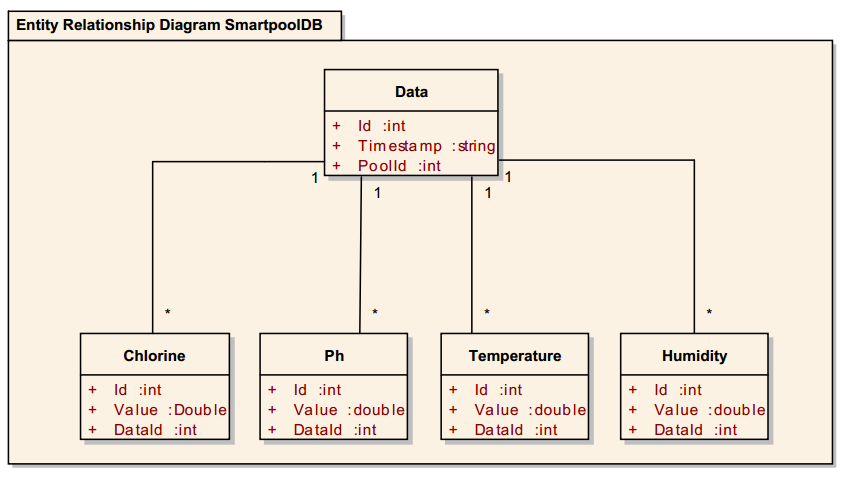
\includegraphics[width=0.8\linewidth]{figs/implementering/datasetentity.png}
	\caption{Data Entity fra ER diagrammet i Visual Studio}
	\label{fig:datasetentity}
\end{figure}

Når \gls{ef} oversætter ER diagrammet til C\# kode og laver scriptet, bliver eksempelvis Chlorine Entity'en til C\# koden vist i listing~\ref{code:chlorinecode}. I dette kodesnit kan man se hvordan \gls{ef} har givet \textit{Chlorine} klassen en \textit{virtual Data}, som et eksempel på lazy loading anvendt.

\begin{minipage}[h]{\linewidth}
\begin{lstlisting}[caption=C\# kode repræsentationen af Chlorine entity.,label=code:chlorinecode]
public partial class Chlorine
{
	public int Id { get; set; }
	public double Value { get; set; }
	public int DataId { get; set; }
	
	public virtual Data Data { get; set; }
}
\end{lstlisting}
\end{minipage}

\begin{figure}
	\centering
	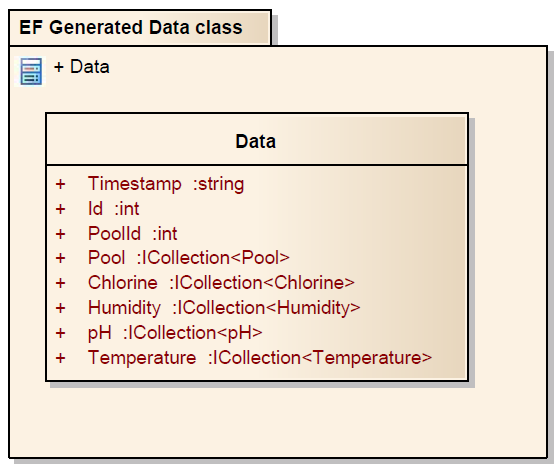
\includegraphics[width=0.5\linewidth]{figs/implementering/efGeneratedData.PNG}
	\caption{Data klassen - Genereret fra Entity Model}
	\label{fig:efGeneratedData}
\end{figure}

\subsection{Implementering af data-access layer}

Entity Frameworket er et \textit{object-relational mapping} framework. Det giver mulighed for at oprette et database-kontekst objekt. Ændringer/indsætning af data sker gennem dette objekt. Når der ønskes en query på databasen gøres det i projektet ved hjælp af en LINQ\footnote{Language Integrated Query} query på en af kontektsobjektets properties. Disse properties er af typen \textit{DbSet<T>} som er en samling af alle entiterne, T i konteksten. Resultatet en af query kan da behandles i en foreach løkke.

For at give et indblik i implementeringen, kan der nedenfor ses kodeudsnit, som tager udgangspunkt i to af projektets user stories, herunder tilføjelse af bruger samt at visning af pooldata.

\subsubsection{Træk pooldata ud}

\textit{"Som bruger vil jeg kunne se de seneste sensor værdier for at kunne få et overblik over poolens tilstand"}\

I de følgende kodeudsnit vises der med tilhørende forklaring hvordan data kan udtages fra databasen. I dette eksempel bruges metoden \textit{GetChlorineData()}, en dybdegående forklaring af alle \textit{Get..Data} metoder kan findes i dokumentationen \todo{reference til dokumentation}.

\begin{lstlisting}[caption=GetChlorineData method - konvertering af DateTime objekter, label=code:getChlorineData]
public List<Tuple<SensorTypes, double>> GetChlorineValues(string poolOwnerEmail, string poolName, int daysToGoBack)
{
	double days = System.Convert.ToDouble(daysToGoBack);
	string now = DateTime.UtcNow.ToString("G");
	string start = DateTime.Parse(now).AddDays(-days).ToString("G");
	...
\end{lstlisting}

På kodeudsnit \ref{code:getChlorineData} vises måden hvorpå et UTC timestamp oprettes. Der benyttes UTC tid da al data gemmes på én server. Det er derfor ligegyldigt hvor i verden en måling bliver foretaget, da dens timestamp vil følge UTC. Det nuværende tidspunkt skal bruges da meningen med funktionen er at returnere alt klor-data der er målt i tidsperioden angivet som \textit{daysToGoBack} parameteren. DateTime \cite{dotnetdatetime} klassen er en del af .NET og indeholder informationer om klokkeslet og dato. Antallet af dage der skal samles informationer om fratrækkes den nuværende DateTime. Derved fås startdatoen til data queryen. Strengen G der medgives som parameter til \textit{ToString}, bevirker at formateringen af tid og dato bliver \textit{dd/MM/yyyy HH:mm:ss}

\begin{lstlisting}[caption=Konvertering tilbage til DateTime objekter,label=code:convertToDateTime]
using (var db = new DatabaseContext())
		{   
			DateTime startTime = DateTime.ParseExact(start, "dd/MM/yyyy HH:mm:ss", System.Globalization.CultureInfo.InvariantCulture);
			DateTime endTime = DateTime.ParseExact(now, "dd/MM/yyyy HH:mm:ss", System.Globalization.CultureInfo.InvariantCulture);

			var chlorineDataQuery = from chlorine in db.ChlorineSet
					where chlorine.Data.Pool.Name == poolName && chlorine.Data.Pool.User.Email == poolOwnerEmail
					select chlorine;

\end{lstlisting}

Som det kan ses på kodeudsnit \ref{code:convertToDateTime} konverteres timestamp strengene til DateTime objekter, hvorefter der bruges LINQ til at lave en forespørgsel på klor-data. Bemærk at der kun hentes klor-data for én specifik bruger og en enkelt af brugerens pools.

\begin{lstlisting}[caption=Iteration over indhentet pool data,label=code:dataIteration]
List<Tuple<SensorTypes, double>> chlorineTuples = new List<Tuple<SensorTypes, double>>();

foreach (var chlorine in chlorineDataQuery)
{
	if(DateTime.Parse(chlorine.Data.Timestamp).CompareTo(endTime) < 0 ||
	DateTime.Parse(chlorine.Data.Timestamp).CompareTo(startTime) > 0)
	{
		chlorineTuples.Add(new Tuple<SensorTypes, double>(SensorTypes.Chlorine, chlorine.Value));
	}
}

return chlorineTuples;
\end{lstlisting}

Returtypen på metoden er en liste af tupler, hvor hver tuple repræsenterer en måling. Som det kan ses på kodeudsnit \ref{code:dataIteration} sammenlignes den data som blev hentet i kodeudsnit \ref{code:convertToDateTime} med de to DateTime objekter, \textit{endTime} og \textit{startTime}. På denne måde gemmes de relevante klor data som tupler i listen.

\subsubsection{Tilføj user}

\textit{"Som bruger vil jeg kunne oprette mig i systemet for at få adgang til systemet"}

I de følgende kodeudsnit vises der med tilhørende forklaringer hvordan en bruger bliver oprettet og gemt i databasen. Der tages udgangspunkt i metoden \textit{AddUser}, som er en del af UserAccess\footnote{Se dokumentationen XXXX} klassen. AddUser metoden kaldes af ConnectionServer klassen \todo{indsæt kodeudsnit af kald her!} som set på figur XXXX.
 
\begin{lstlisting}[caption=User laves lokalt hvorefter User's navne properties sættes, label=code:adduser1]
public bool AddUser(string fullname, string email, string password)
{
	...
	//Checks for existing user and valid name
	...
	
	User user;

	string[] names = fullname.Split(' ');

	if (names.Length <= 2)
	{
		user = new User() { Firstname = names[0], Lastname = names[1], Email = email, Password = password };
	}
	else
	{
		user = new User() { Firstname = names[0], Middelname = names[1], Lastname = names[2], Email = email, Password = password };
	}
\end{lstlisting}

Som det kan ses på kodeudsnit \ref{code:adduser1} Oprettes en user først lokalt, hvorefter user objektets navne, password og email properties sættes. En User's navn opdeles i Firstname, Middlename og Lastname strings. 

\begin{lstlisting}[caption=User objektet tilføjes i database konteksten hvorefter der gemmes på selve databasen,label=code:adduser2]
	using (var db = new DatabaseContext())
	{
		db.UserSet.Add(user);
		db.SaveChanges();
	}

	return true;
}
\end{lstlisting}

Når der skal foretages ændringer på databasen, oprettes et database kontekst objekt hvor ændringerne gemmes på. Derefter kaldes \textit{db.SaveChanges()} metoden, som gemmer ændringerne på selve databasen. Se kodeudsnit \ref{code:adduser2} for eksempel på brugen af database konteksten med \textit{using} direktivet.

